%\documentclass[a4paper]{article}
%\usepackage[T1]{fontenc}
%\usepackage[utf8]{inputenc}
%\usepackage[italian]{babel}
%\usepackage{amssymb}
%\usepackage{amsmath}
%\usepackage{hyperref}
%\usepackage{amsthm}
%\usepackage{graphicx}
\documentclass[journal, a4paper]{IEEEtran}
\usepackage[italian]{babel}
\usepackage{booktabs}
\usepackage{siunitx}%Questo serve a caricare il pacchetto delle unità di misura del sistema internazionale%
\usepackage[utf8]{inputenc}
\usepackage{graphicx} 
\usepackage{url}
\usepackage{amsmath}
\usepackage{gensymb}
\usepackage{longtable}
\usepackage{keyval}
\usepackage{xcolor}
\usepackage{caption}
\usepackage{tikz}
\usepackage{circuitikz}
\usepackage{authblk}
%\usepackage{hyperref}

\begin{document}


% Define document title and author
	\title{Tecnologie Digitali - Logbook Week 5}
	\author[1]{Salvatore Bottaro}
		\author[2]{Lorenzo M. Perrone}
		\affil[1]{\texttt{salvo.bottaro@hotmail.it}}
		\affil[2]{\texttt{lorenzo.perrone.lmp@gmail.com}}
	\markboth{Tecnologie Digitali - Di Lieto}{}
	\maketitle
	
\begin{abstract}
	Logbook di laboratorio di Tecnologie Digitali, a.a. 2015/2016. Week 5.
\end{abstract}

\section{Meccanismo e caratteristica I-V del LED}
In un LED il meccanismo di emissione della luce avviene in seguito ad un processo di ricombinazione fra le cariche presenti nella banda di conduzione e quelle nella banda di valenza. Il processo porta all'emissione di un fotone di energia:
\begin{equation}
\Delta E = h \, \frac{c}{\lambda}
\end{equation}

Dal momento che $hc$ = 1240 eV $\cdot$ nm, questo suggerisce una regola mnemonica per convertire in eV le lunghezze d'onda espresse in nm:

\begin{equation}
\Delta E = \frac{1240}{\lambda(nm)} \; eV
\end{equation}

Ad esempio nel caso di luce blu, $\lambda = 470$ nm, si ottiene $\Delta E \approx 2.6$ eV.\\
Per una prima stima della costante di Planck abbiamo impiegato un LED rosso (645 nm) modello HLMP-C115, realizzando sulla breadboard il circuito dello schema in figura \ref{fig:led_circ}.\\

\begin{figure}[htp]
\centering
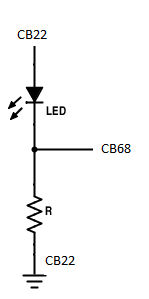
\includegraphics[scale=.6]{led_circ}
\caption{Schema del circuito realizzato sula breadboard. Sono indicate anche le porte della scheda di acquisizione impiegate.}
\label{fig:led_circ}
\end{figure}

Dal datasheet di HLMP-C115 è possibile leggere il massimo valore per la corrente diretta:
\begin{equation}
I_F = 30\, mA
\end{equation}

che pone un vincolo sul valore minimo della resistenza R. Questo può essere dedotto osservando la caratteristica I-V del LED riportata nel datasheet (figura \ref{fig:c115car}).

\begin{figure}[htp]
\centering
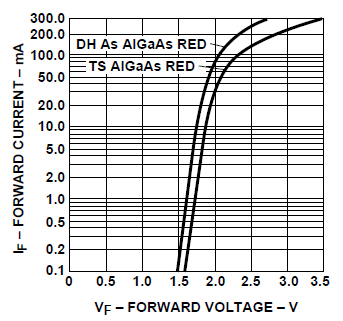
\includegraphics[scale=.6]{IF-VF}
\caption{Curva caratteristica del LED che si può leggere nel datasheet. Il modello da noi impiegato corrisponde al DH As AlGaAs RED.}
\label{fig:c115car}
\end{figure}

Come si vede se V è la tensione di ingresso, $\Delta$V la tensione diretta ai capi del LED in funzione della corrente I, si ha che R vale:
\begin{equation}
R = \frac{V-\Delta V}{I}
\end{equation}

Per V = 10 V (massima tensione generata dalla scheda), I = $I_F$, $\Delta$V $\approx$ 1.8 V (tensione diretta a cui la corrente che scorre nel LED è quella massima) si ottiene:
\begin{equation}
R_{min} \approx 275 \, \Omega
\end{equation}

Nell'esperienza abbiamo impiegato una resistenza R = 470 $\pm$ 0.8 $\%$. In queste condizioni è possibile stimare sempre dalla curva di figura \ref{fig:c115car} che applicando una tensione di ingresso da 10 V la corrente massima nel circuito risulti circa 18 mA. Infatti bisogna individuare il punto di intersezione fra la curva caratteristica del LED e la retta V = 10 V - R$\cdot$I, che si vede facilmente essere compreso in 1.5 V $\leq$ V $\leq$ 2 V e 1.7 mA $\leq$ I $\leq$ 1.8 mA.\\

Abbiamo infine montato il circuito di figura \ref{fig:led_circ} sulla breadboard. Con il VI \textbf{\texttt{Vin$\_$Vout$\_$2015}} abbiamo impostato diversi valori della tensione di ingresso, ricavando da $V_{out}$ il valore della corrente che scorreva nel LED. I valori misurati sono riportati in tabella \ref{tab:firstmis}.

\begin{table}[htp]
\centering
\caption{Prime misure della corrente nel LED. I valori di $V_{in}$ riportati sono quelli impostati nel VI.}
\label{tab:firstmis}
\begin{tabular}{|c|c|c|}
\hline 
$V_{in}$ (V)& $V_{out}$ (V)& I (mA)\\ 
\hline 
1 & 0 & 0 \\ 
\hline 
2 & 0.4053(7) & 0.862(7) \\ 
\hline 
3 & 1.3289(11) & 2.83(2) \\ 
\hline 
4 & 2.297(4) & 4.89(4) \\ 
\hline 
5 & 3.299(8) & 7.02(6) \\ 
\hline 
\end{tabular}
\end{table} 
 
Abbiamo poi effettuato delle misure impostando $V_{in}$ fra 1 V e 2 V, poiché si è visto che il LED si accende proprio in questo intervallo. Le misure effettuate sono riportate in tabella \ref{tab:secmis}.

\begin{table}[htp]
\centering
\caption{Determinazione della corrente di prima accensione del LED.}
\label{tab:secmis}
\begin{tabular}{|c|c|c|c|}
\hline 
$V_{in}$ (V)& $V_{out}$ (mV)& $V_{LED}$ (V) & I ($\mu$A)\\ 
\hline 
1.3 & 0 & 0 & 0 \\ 
\hline 
1.35 & 2.44(0) & 1.348 & 5.19(4) \\ 
\hline 
1.4 & 4.88(6) & 1.39 & 10.38(8) \\ 
\hline 
1.5 & 22.1(4) & 1.4779 & 47.0(4) \\ 
\hline 
\end{tabular} 
\end{table} 
 
In particolare abbiamo individuato il punto di prima accensione del LED per $V_{in}$ = 1.35 V, cui corrisponde una \textit{forward voltage} $V_f$ = 1.348(BOH) e una corrente $I_f$ = 5.19(4) $\mu$A. Per quanto riguarda l'errore riportato per alcuni valori di $V_{out}$, il fatto che in qualche caso si sia riportato 0 è dovuto al fatto che l'errore calcolato dal VI \textbf{\texttt{Vin$\_$Vout$\_$2015}}, ovvero la deviazione standard su un certo numero di misure, era più piccolo del minimo valore riportabile. Eseguendo infatti la stessa misura con \textbf{\texttt{Traccia$\_$Vin$\_$Vout}} nelle stesse condizioni con fondoscala 0.05 V, i punti ottenuti avevano la stessa ordinata a parte 2 punti che differivano dagli altri di COME SI CHIAMA?

\subsection{Stima di \textit{h}} 
Tramite il VI \textbf{\texttt{Traccia$\_$Vin$\_$Vout}} abbiamo campionato l'equivalente della caratteristica I-V del LED. Infatti come si vede in figura \ref{fig:ledcar}, si è misurata la tensione $V_{out}$ in funzione di $V_{in}$, da cui ovviamente è possibile risalire alla corrente che scorre nel LED semplicemente dividendo per la resistenza R. \\

\begin{figure}[htp]
\centering
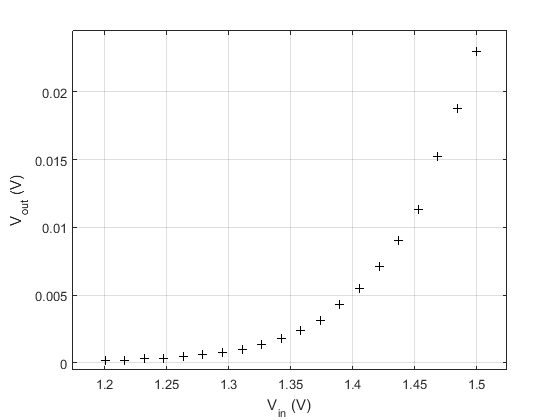
\includegraphics[scale=.6]{graph_led}
\caption{Grafico dei dati sperimentali di $V_{out}$ in funzione di $V_{in}$ equivalente alla caratteristica I-V.}
\label{fig:ledcar}
\end{figure}

Dal grafico si vede come la corrente comincia a crescere rapidamente per $V_{out}$ = 1.37 V $\pm$ 0.02 V, compatibile con il valore trovato per la tensione di prima accensione del LED, e che può essere presa come stima della $V_{gap}$ fra la banda di conduzione e di valenza. Da qui, tramite:
\begin{equation}
h = \frac{\lambda e V_{gap}}{c}
\end{equation}

è possibile fornire una prima stima di h. Utilizzando i valori di \textit{e} e \textit{c} universalmente accettati forniti da \texttt{CODATA}:
\begin{equation}
e = 1.6021766208(98) \cdot 10^{-19} \, C
\end{equation}
\begin{equation}
c = 299 792 458 \, \frac{m}{s}
\end{equation}

mentre come valore della lunghezza d'onda emessa dal diodo abbiamo preso $\lambda$ = 645 nm $\pm$ 12 nm, ovvero il valore di picco e come errore la HWHM che si può dedurre dal grafico dell'intensità relativa in funzione della lunghezza d'onda che si trova nel datasheet. Si ottiene così:
\begin{equation}
h_{ext} = (4.7 \pm 0.2) \cdot 10^{-34} Js
\end{equation}

Come si può notare, il valore stimato differisce di circa il 30 $\%$ da quello attualmente accettato. Difatti il metodo impiegato si basa su una scelta soggettiva del valore di soglia per la stima di $V_{gap}$ nella caratteristica I-V del LED. Tuttavia nonostante ciò la stima è ragionevole.

\section{Misura di h}

La criticità più evidente del metodo esposto nella sezione precedente per ottenere il valore di \textit{h} risiede nella valutazione arbitraria e soggettiva del valore della tensione $V_G$ di "ginocchio", termine poco appropriato, a cui si verifica un evidente aumento della corrente che scorre nel LED (o, come nel nostro caso, della tensione in uscita $V_{out}$).\\

Per effettuare una misura un po' più accurata della costante di Planck, possiamo fare riferimento al modello della distribuzione di Boltzmann in energie dei portatori di carica. Infatti, la corrente di saturazione $I_S$ è proporzionale proprio alla densità dei portatori, e dunque $I_S \propto \exp(V_G/kT)$, a meno di un coefficiente moltiplicativo $I^*(T)$ che tiene conto del materiale della giunzione e del processo di fabbricazione, e che noi stiamo trascurando supponendo (si vedrà se a ragione) che i LED a nostra disposizione appartengano tutti alla stessa \textit{famiglia}.\\
Possiamo, dunque, riscrivere l'equazione di Shockley nella seguente forma a noi più comoda:

\begin{equation}\label{new_shockley}
I(V)  \propto \exp{\frac{V-V_G}{V_T}} ; \; \boxed{con V_T = kT}
\end{equation}

In altre parole, fissata la stessa corrente per tutti i LED in esame, la differenza $V-V_G$ è costante. Quindi possiamo riportare $V$ (anzi, $qV/c$) in ordinata, e $\lambda^{-1}$ in ascissa, per ottenere una retta la cui pendenza corrisponderà proprio a $h$. Per essere più precisi: scegliendo di plottare sull'asse delle y $V_{out}, V_G, V_F$ (dove $V_F$ sta per \textit{forward} e nel nostro caso $V_F = V_{in} - V_{out}$), l'unico risultato sarà quello di shiftare verso l'alto o il basso la retta di fit, cambiandone l'intercetta ma non il coefficiente angolare.\\

Scegliamo quindi un valore opportuno della corrente, che non sia troppo alto in modo da ridurre al minimo comportamenti resistivi del LED, come prima prova è stata scelta $I = 20 \mu \si{A}$; plottiamo quindi la curva I-V per tutti i diodi a nostra disposizione e troviamo per ciascuno il valore $V(I=20 \mu \si{A})$.\\

Prima di procedere riportando i dati ottenuti, è opportuno fare alcune precisazioni:

\begin{itemize}
\item Poichè il VI da noi impiegato per l'acquisizione dati è il \textbf{Vin\_Vout\_2015}, i canali \textsc{cb22} e \textsc{cb68} ci hanno permesso di misurare la caratteristica $V_{out} - V_{in}$ e non quella $I-V$. Tuttavia, a meno di una costante moltiplicativa pari alla resistenza di carico $R$ nota, la corrente $I \propto V_{out}$, per cui non ci sono particolari controindicazioni.

\item Nel corso dell'acquisizione dati, il calcolo del valore $V_{in}$ corrispondente alla corrente I di $20 \mu $A, è stato effettuato "visivamente" individuando gli intervalli $[V_- , V_+]$ entro cui eravamo certi di trovare la $V_{20}$ (poichè $I(V_-) < 20 \mu \si{A} < I(V_+)$),e prendendo quindi come errore sulla tensione la semidifferenza. Nella rielaborazione dei dati, invece, le curve esponenziali I-V sono state interpolate per mezzo di Octave, tramite la funzione \textbf{polyfit}, con un polinomio di 25esimo grado, da cui è stata ricavata l'intercetta con il valore di $I = 20 \mu $A usando opportunamente la funzione \textbf{root}. Ad ogni modo, l'errore sulle tensioni così ottenute è stato comunque lasciato pari a quello trovato in precedenza, dal momento che un'interpolazione, per quanto ottimale, non può certamente aumentare la precisione dei dati effettivamente acquisiti.

\item Per quanto riguarda le lunghezze d'onda $\lambda$, si è deciso di utilizzare come incertezza indicativa la differenza fra il valore di \textit{peak} e quello \textit{dominant}.

\item Per i LED \textsc{lpk376, led365, led880} l'interpolazione falliva in maniera evidente riportando un errore di singolarità di una matrice impiegata dall'algoritmo. Per ottenere dei risultati molto più accettabili, si è scelto di impiegare un polinomio di 15esimo grado.

\item Per fare il fit, si è propagato l'errore relativo delle lunghezze d'onda sulle y, dal momento che questo non era per nulla trascurabile rispetto agli errori delle tensioni.
\end{itemize}

Riportiamo nella tabella seguente i LED da noi utilizzati e le loro lunghezze d'onda:

{
\centering

\begin{tabular}{|c|c|}
\hline \textbf{LED} & \textbf{$\lambda$ (nm)} \\ 
\hline HLMPC115 & 645 $\pm$ 8 \\ 
\hline HLMPC315 & 587 $\pm$ 6 \\ 
\hline LA3366 & 622 $\pm$ 7 \\ 
\hline LB3333 & 477 $\pm$ 6 \\ 
\hline LED450 & 450 $\pm$ 5 \\ 
\hline LO3336 & 611 $\pm$ 5 \\ 
\hline LPK376 & 566 $\pm$ 6 \\ 
\hline LS3336 & 639 $\pm$ 6 \\ 
\hline TLIHC4405 & 575 $\pm$ 7 \\ 
\hline WP9294 & 471 $\pm$ 5 \\ 
\hline LED365 & 365 $\pm$ 3 \\ 
\hline LED880 & 880 $\pm$ 5 \\ 
\hline 
\end{tabular} 


}

\subsection{Corrente $I = 20 \mu \si{A}$}

Possiamo ora riportare in Figura (\ref{fig:costante_planck_20ua}) i risultati del fit per la corrente $I = 20 \mu \si{A}$.

\begin{figure}
\centering
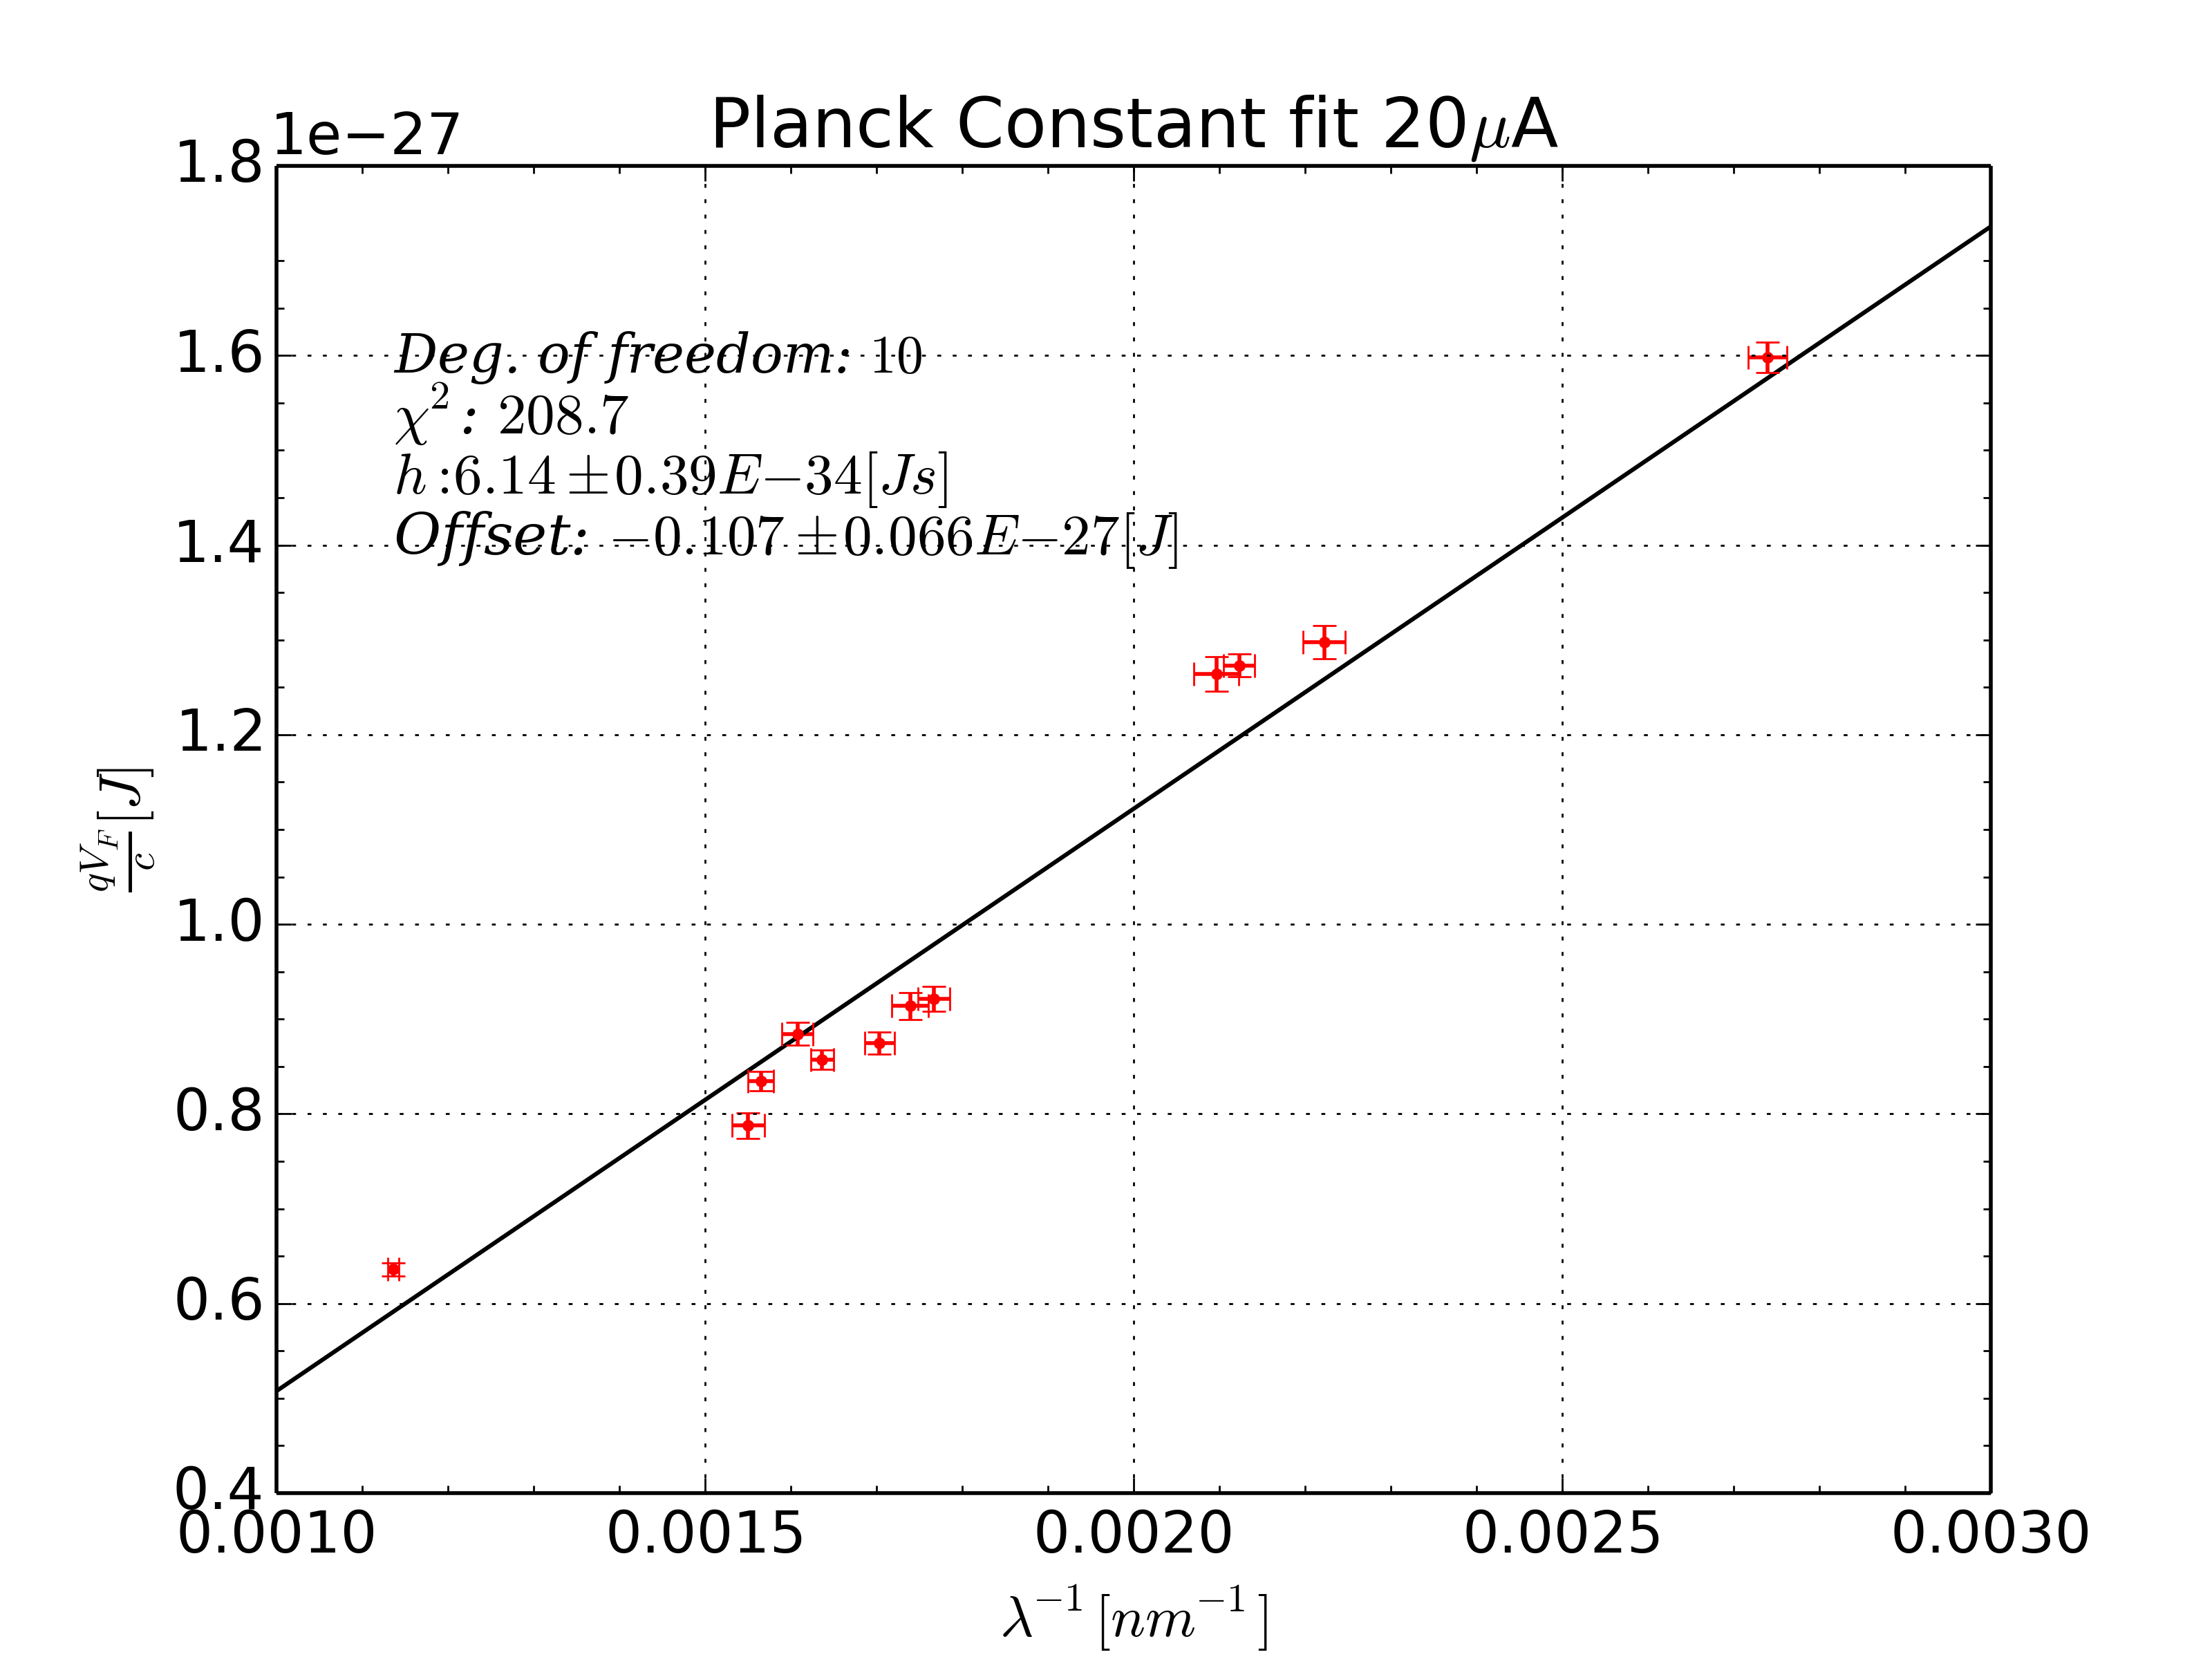
\includegraphics[width=0.9\linewidth]{./costante_planck_20ua}
\caption{Plot e fit delle energie eV/c in funzione del reciproco della lunghezza d'onda.}
\label{fig:costante_planck_20ua}
\end{figure}

Il valore ottenuto di h con questo primo fit è dunque $(6.14 \pm 0.39 ) \, E-34 \, Js$, non troppo distante da quello noto. Possiamo subito notare che i LED a nostra disposizione si dividono in maniera piuttosto netta fra un gruppo nutrito con lunghezze d'onda comprese fra 550-650 nm (nella parte centrale del grafico), un altro meno numeroso con lunghezze d'onda di circa 450-470 nm, e infine due LED estremali a 350nm (ultravioletto) e 880nm (NIR).\\
Oltretutto, la questione risulta ancora più evidente dal momento che \underline{tutti} i LED appartenenti ak gruppo "di mezzo" sono situati sotto la retta di fit, mentre i rimanenti sono al di sopra di questa.\\
Inizia a sorgere il dubbio che i LED impiegati non appartengano alla stessa "famiglia", per quanto riguarda i materiali della giunzione, e se questo fosse vero, cadrebbe una delle ipotesi che abbiamo posto nella derivazione della (\ref{new_shockley}).\\

Per studiare meglio i nostri LED, tracciamo un grafico con le caratteristiche I-V in scala semilogy, per verificare la presenza di differenze nella pendenza delle rette risultanti, cosa che implicherebbe una diversità delle costanti moltiplicative agli esponenziali delle equazioni di Shockley.

\subsection{Caratteristica I-V}

In Figura \ref{fig:tuttiled} riportiamo la caratteristica I-V dei LED in uso.

\begin{figure}
\centering
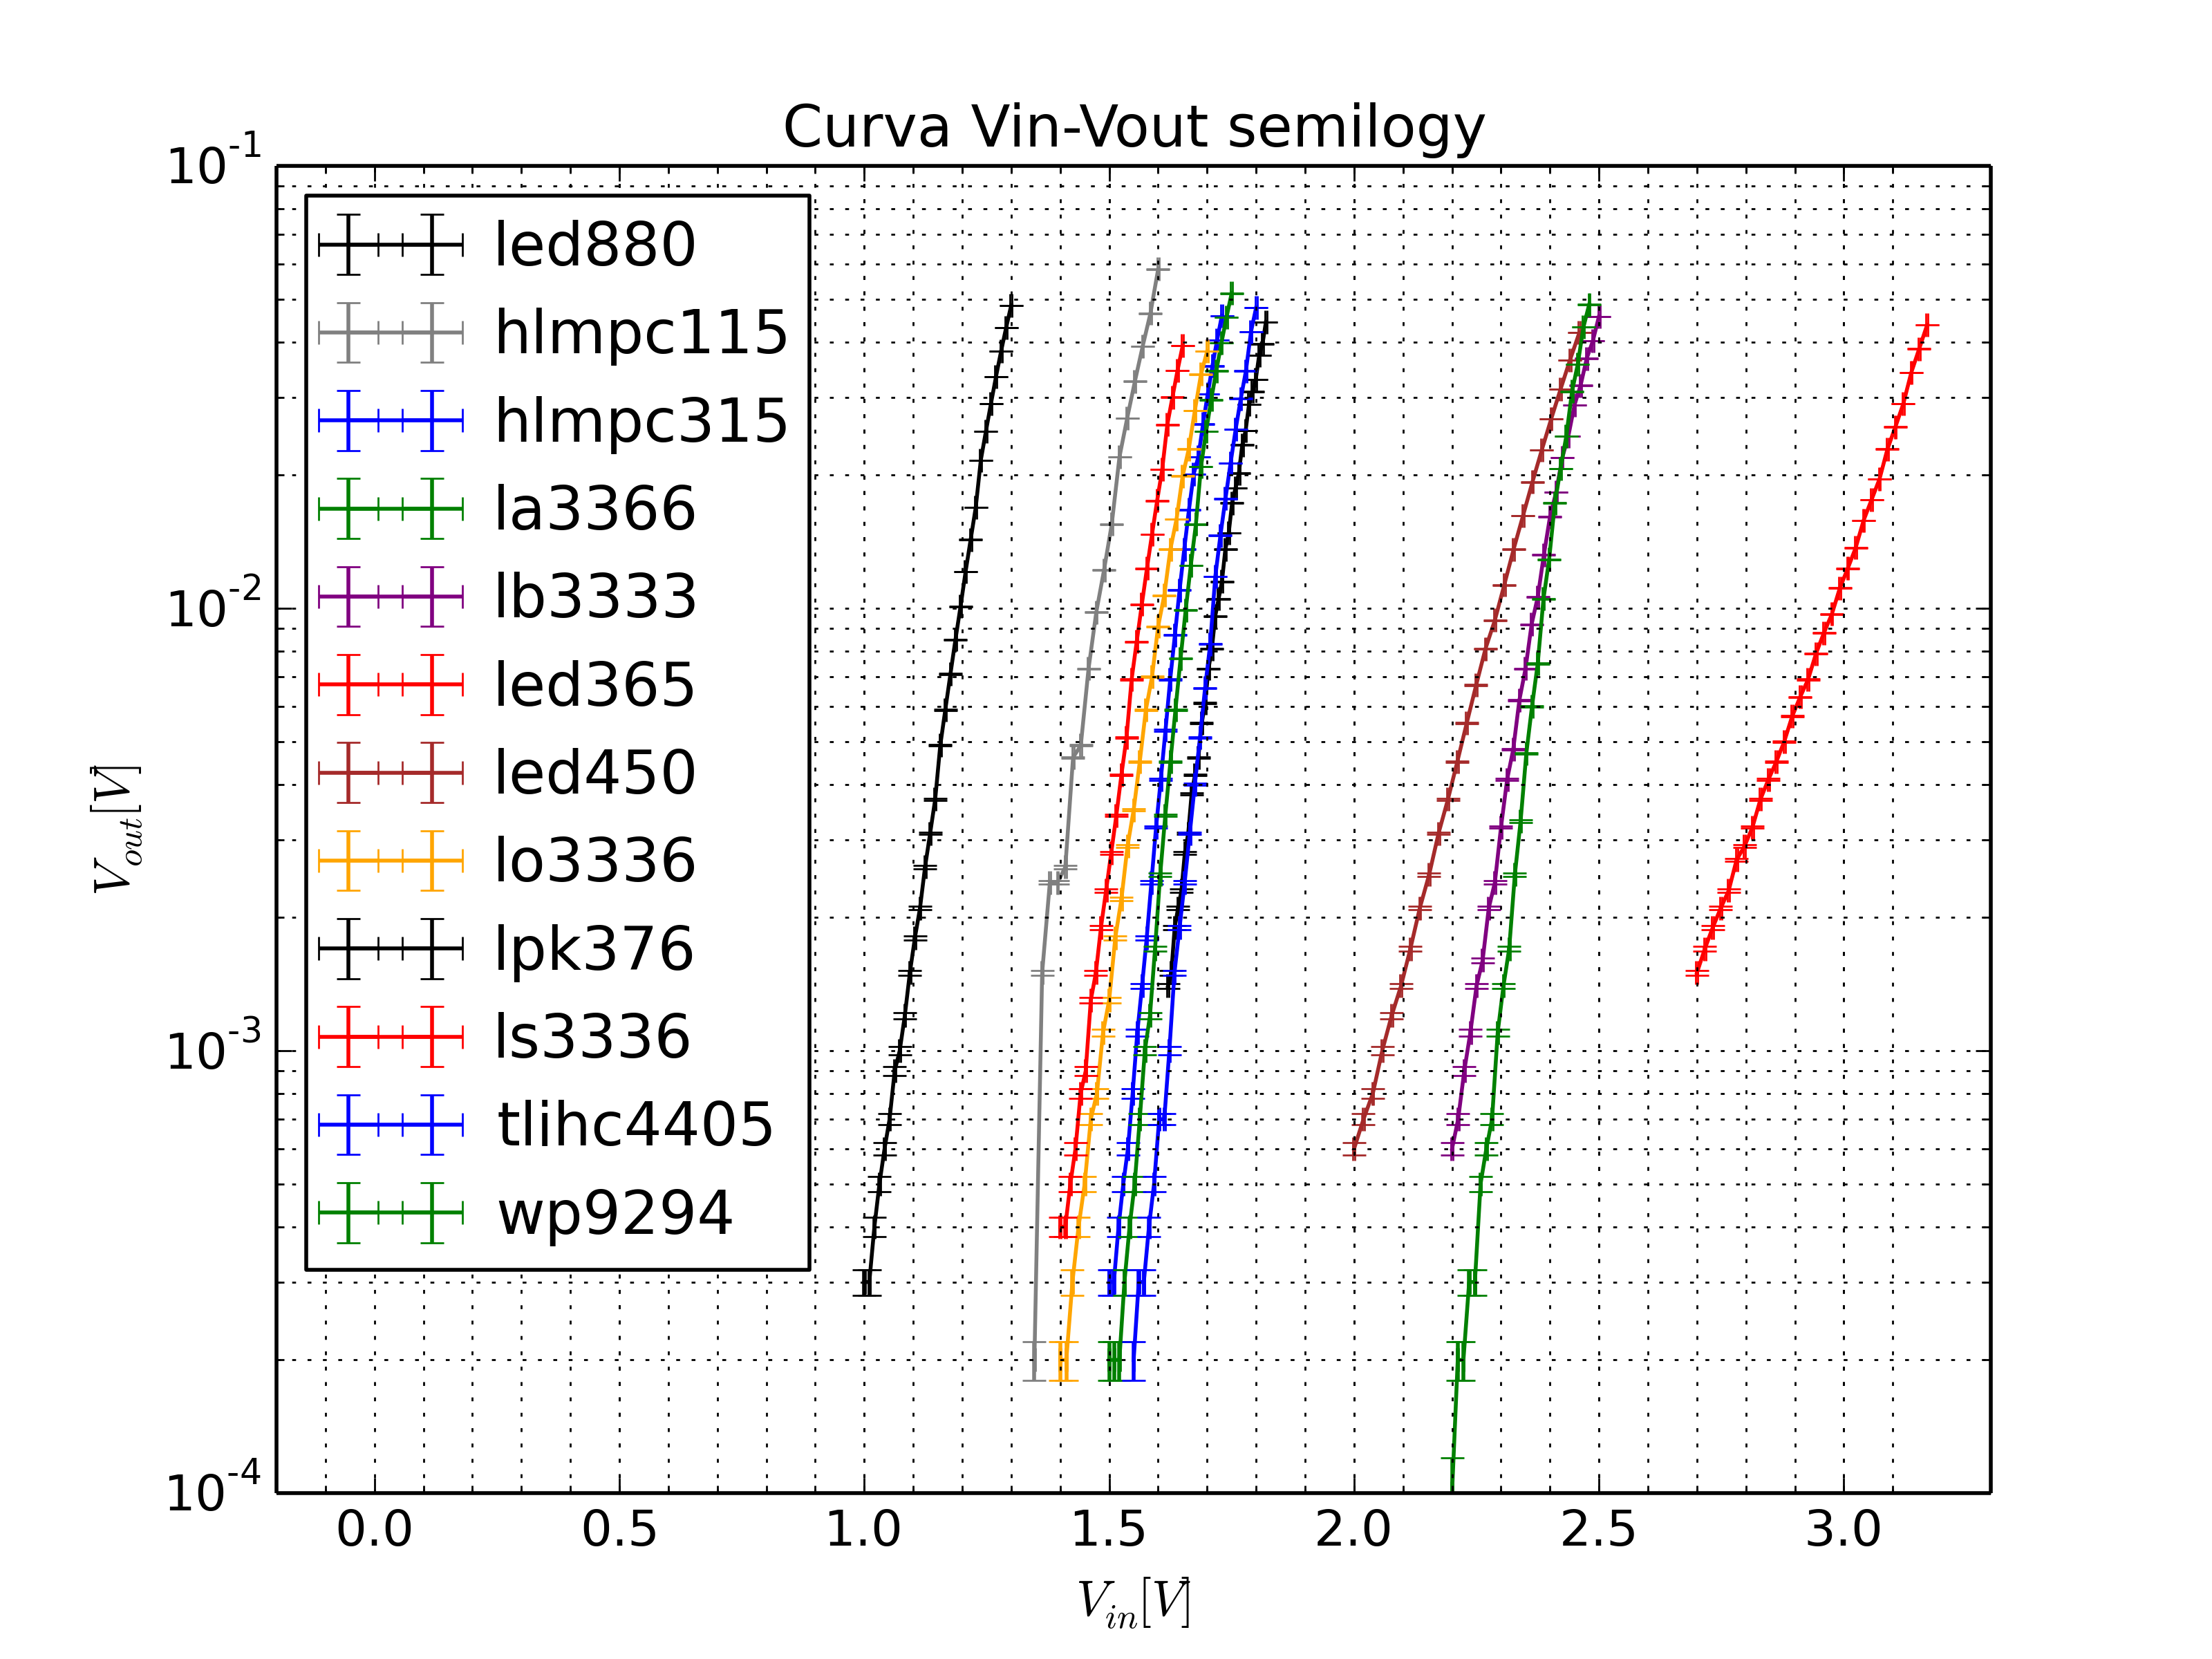
\includegraphics[width=1\linewidth]{./tuttiled}
\caption{Caratteristica I-V dei LED in scala semilogy: si notino le differenze nelle pendenze di alcune delle rette riportate.}
\label{fig:tuttiled}
\end{figure}
 
Come si nota dal grafico, e come avevamo già ipotizzato, nel nostro set di LED ne sono presenti alcuni con caratteristiche sensibilmente diverse fra loro: sicuramente il \textsc{led365}, \textsc{led450}, e evidenziamo inoltre anche un comportamento non proprio ottimale del \textsc{hlmpc115}.\\

\begin{figure}[h]
\centering
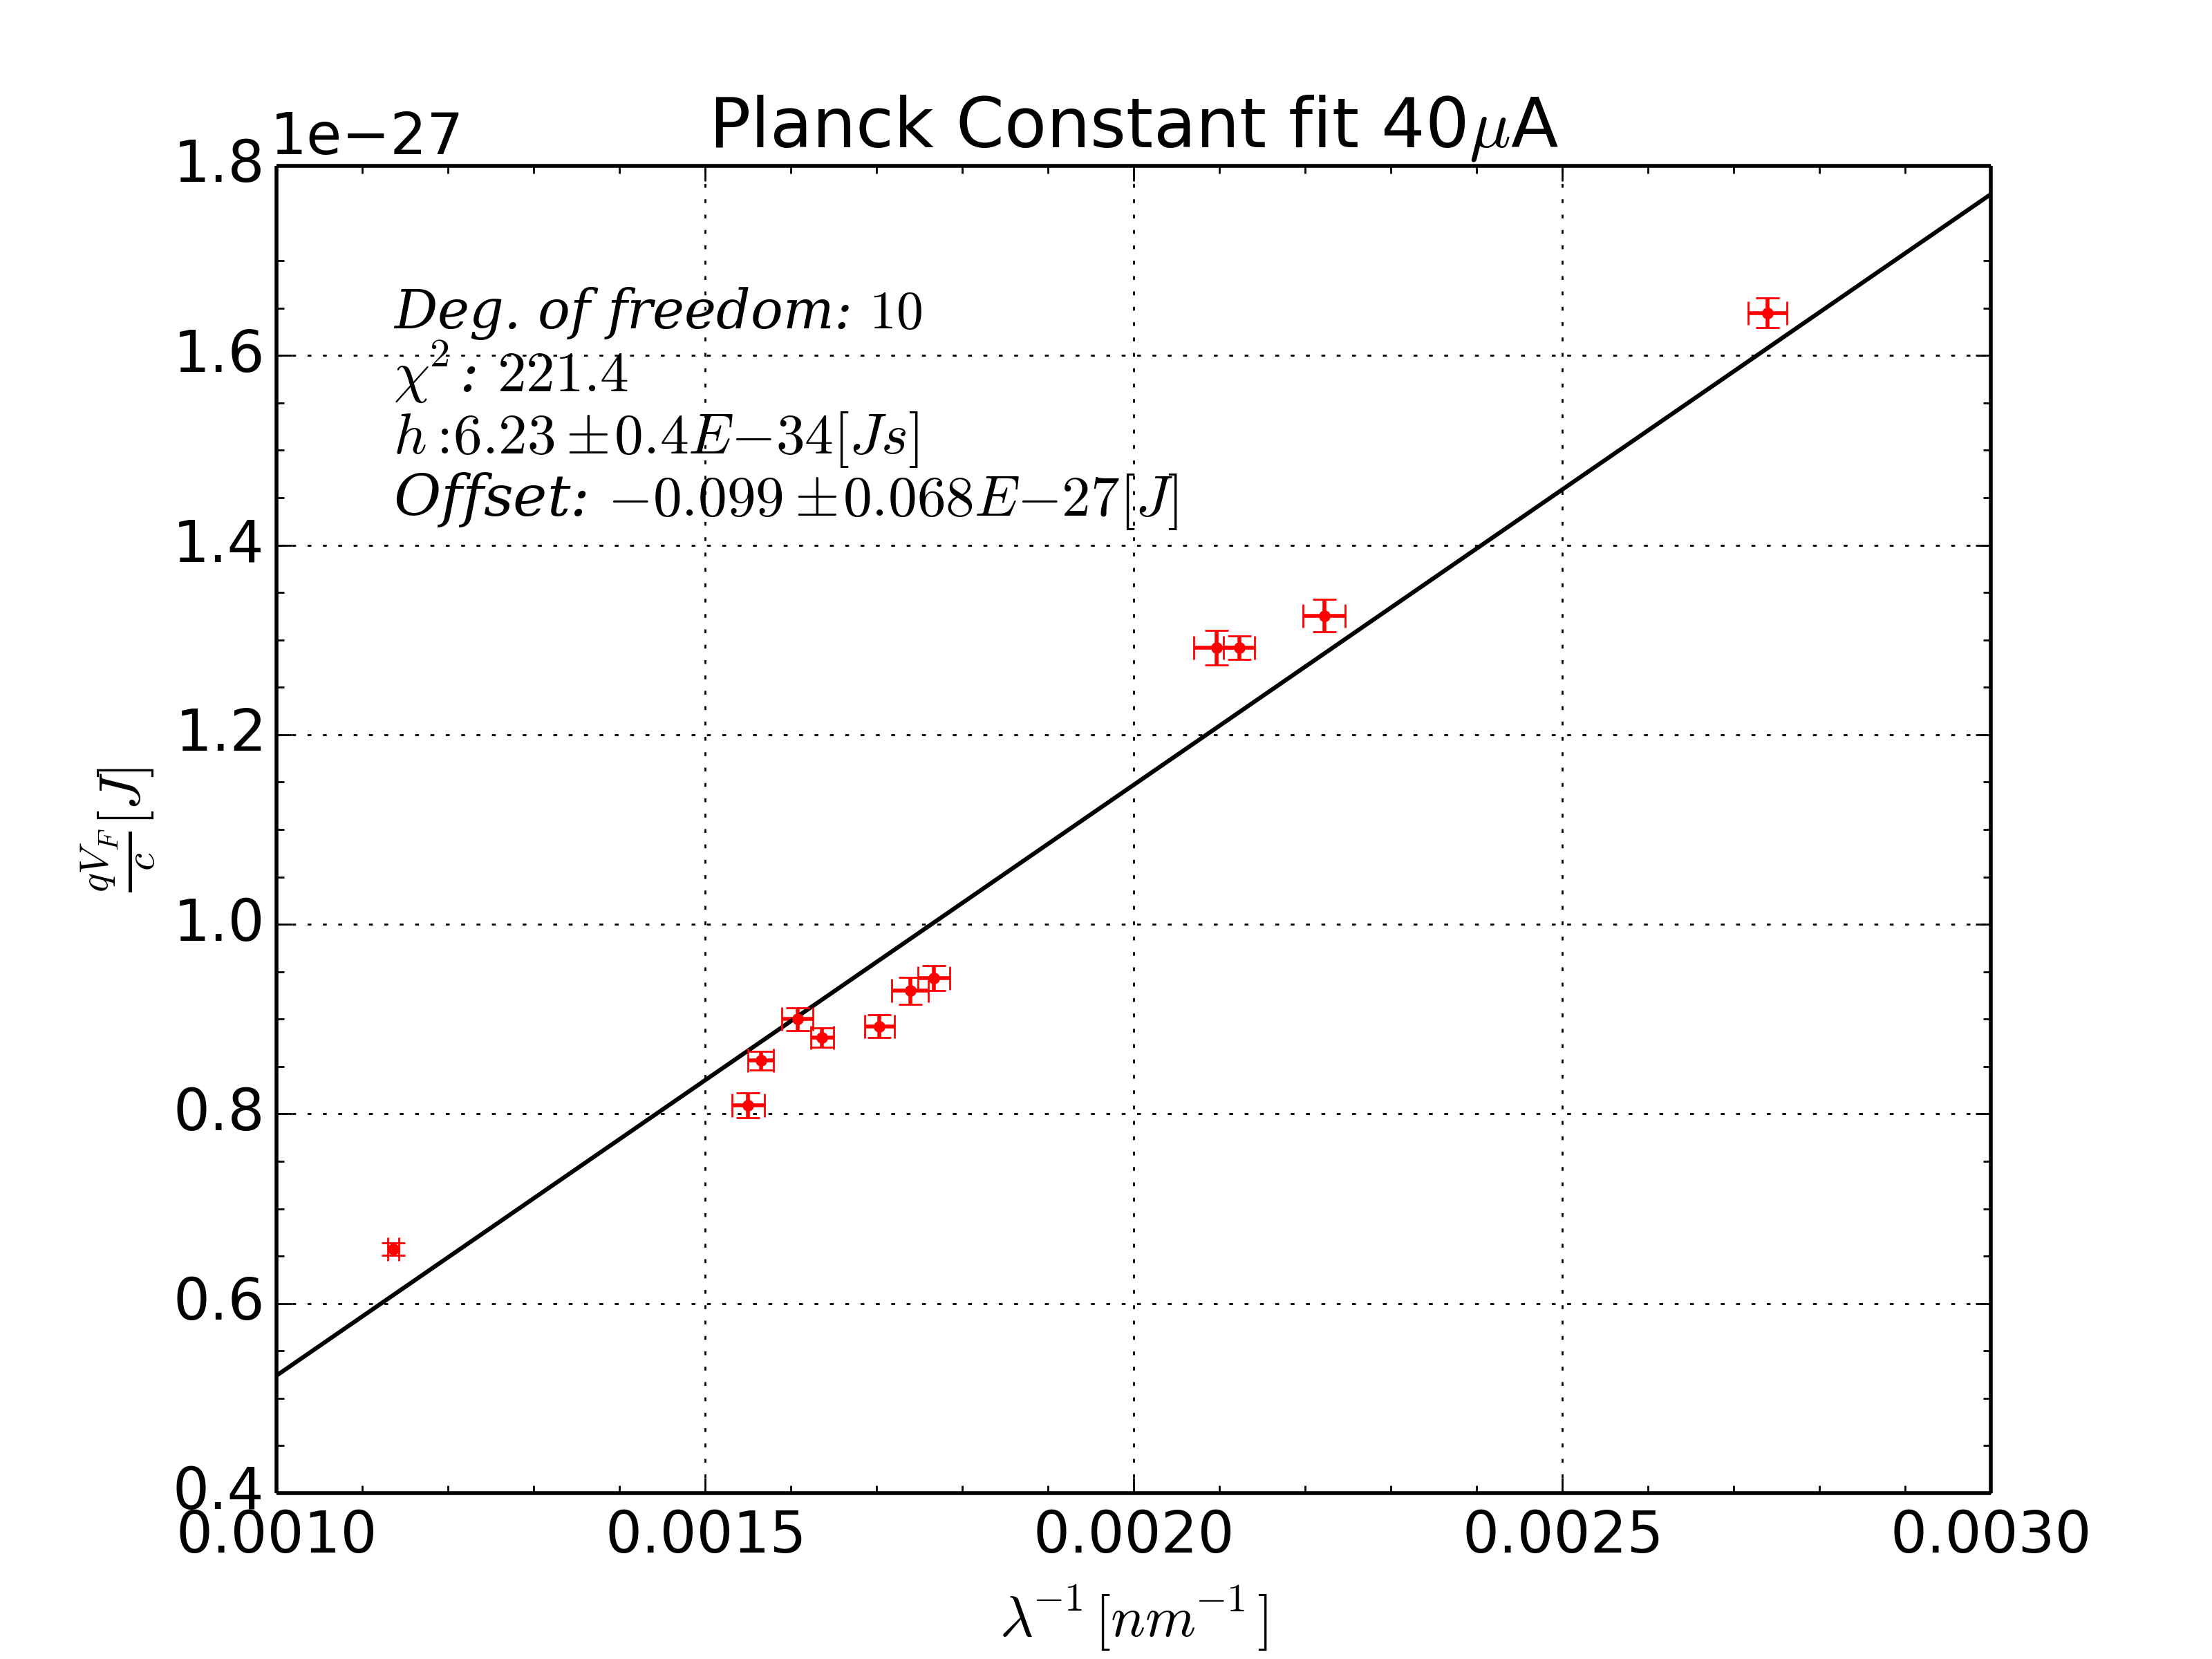
\includegraphics[width=0.9\linewidth]{./costante_planck_40ua}
\caption{Fit delle energie di gap in funzione del reciproco della lunghezza d'onda - 40 $\mu$A}
\label{fig:costante_planck_40ua}
\end{figure}

Per questi motivi, può essere interessante provare a ripetere il procedimento effettuato in precedenza scegliendo dei valori diversi della corrente: se tutti i LED appartenessero alla stessa "famiglia" questo non dovrebbe comportare nessun cambiamento nel fit dei valori interpolati. Tuttavia, dal momento che alcuni seguono caratteristiche I-V differenti, allora sembra plausibile che, tagliando le rette con valori di corrente diversi, anche i risultati dei fit potranno distribuirsi non uniformemente.\\

I valori di corrente scelti sono stati: $20 \mu $A (già analizzato), $40 \mu $A, $60 \mu $A, $80 \mu $A.

\subsection{Corrente $I = 40 \mu \si{A}$}

Si riportano in Figura (\ref{fig:costante_planck_40ua}) i risultati del fit con $I = 40 \mu $A.


Il valore ricavato dal fit della costante di Planck è $6.23(40) \, E-34 \si{Js}$, di poco più prossimo al valore noto.

\subsection{Corrente $I = 60 \mu \si{A}$} 

Si riportano in Figura \ref{fig:costante_planck_60ua}() i risultati del fit con $I = 60 \mu $A.

\begin{figure}
\centering
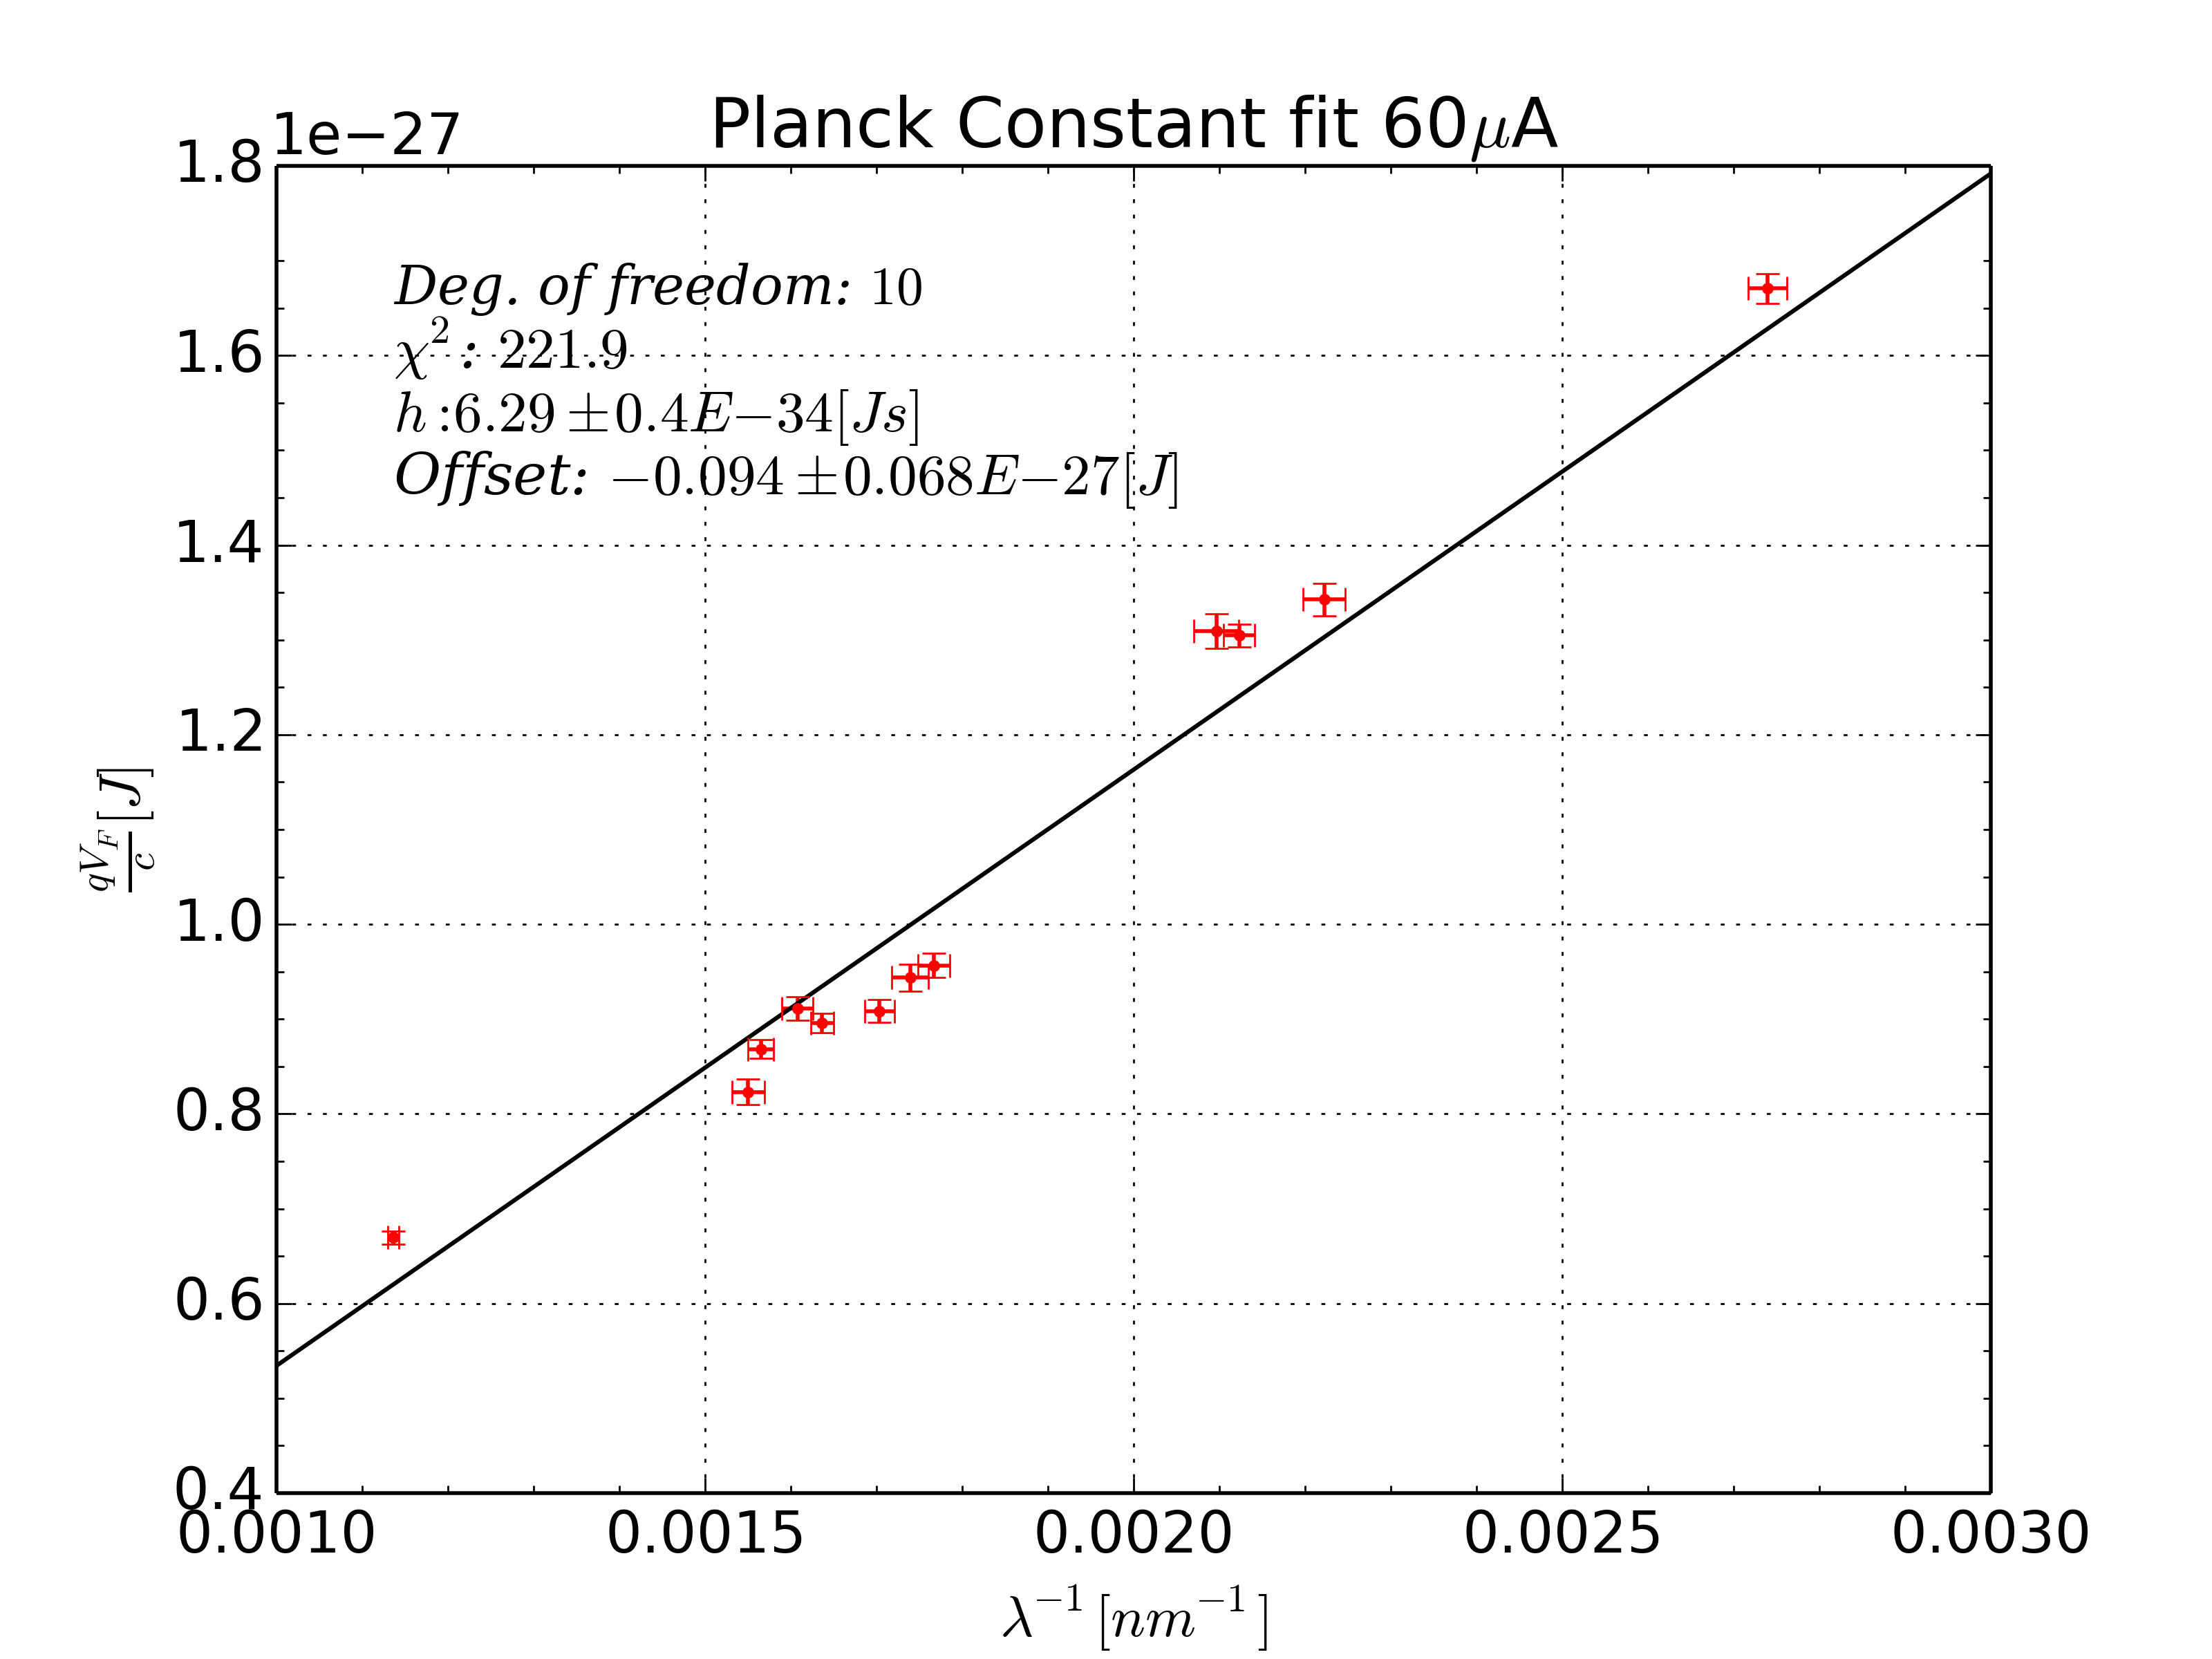
\includegraphics[width=0.9\linewidth]{./costante_planck_60ua}
\caption{Fit delle energie di gap in funzione del reciproco della lunghezza d'onda - 60 $\mu$A}
\label{fig:costante_planck_60ua}
\end{figure}

Il valore ricavato dal fit della costante di Planck è $6.29(40) \, E-34 \si{Js}$. Sembra evidenziarsi un \textit{lieve} aumento del valore di \textit{h}. Notiamo inoltre che adesso il valore conosciuto rientra in un $\sigma$ dell'incertezza del valore restituito dal fit.

\subsection{Corrente $I = 80 \mu \si{A}$}


Si riportano in Figura (\ref{fig:costante_planck_80ua}) i risultati del fit con $I = 80 \mu $A.

\begin{figure}
\centering
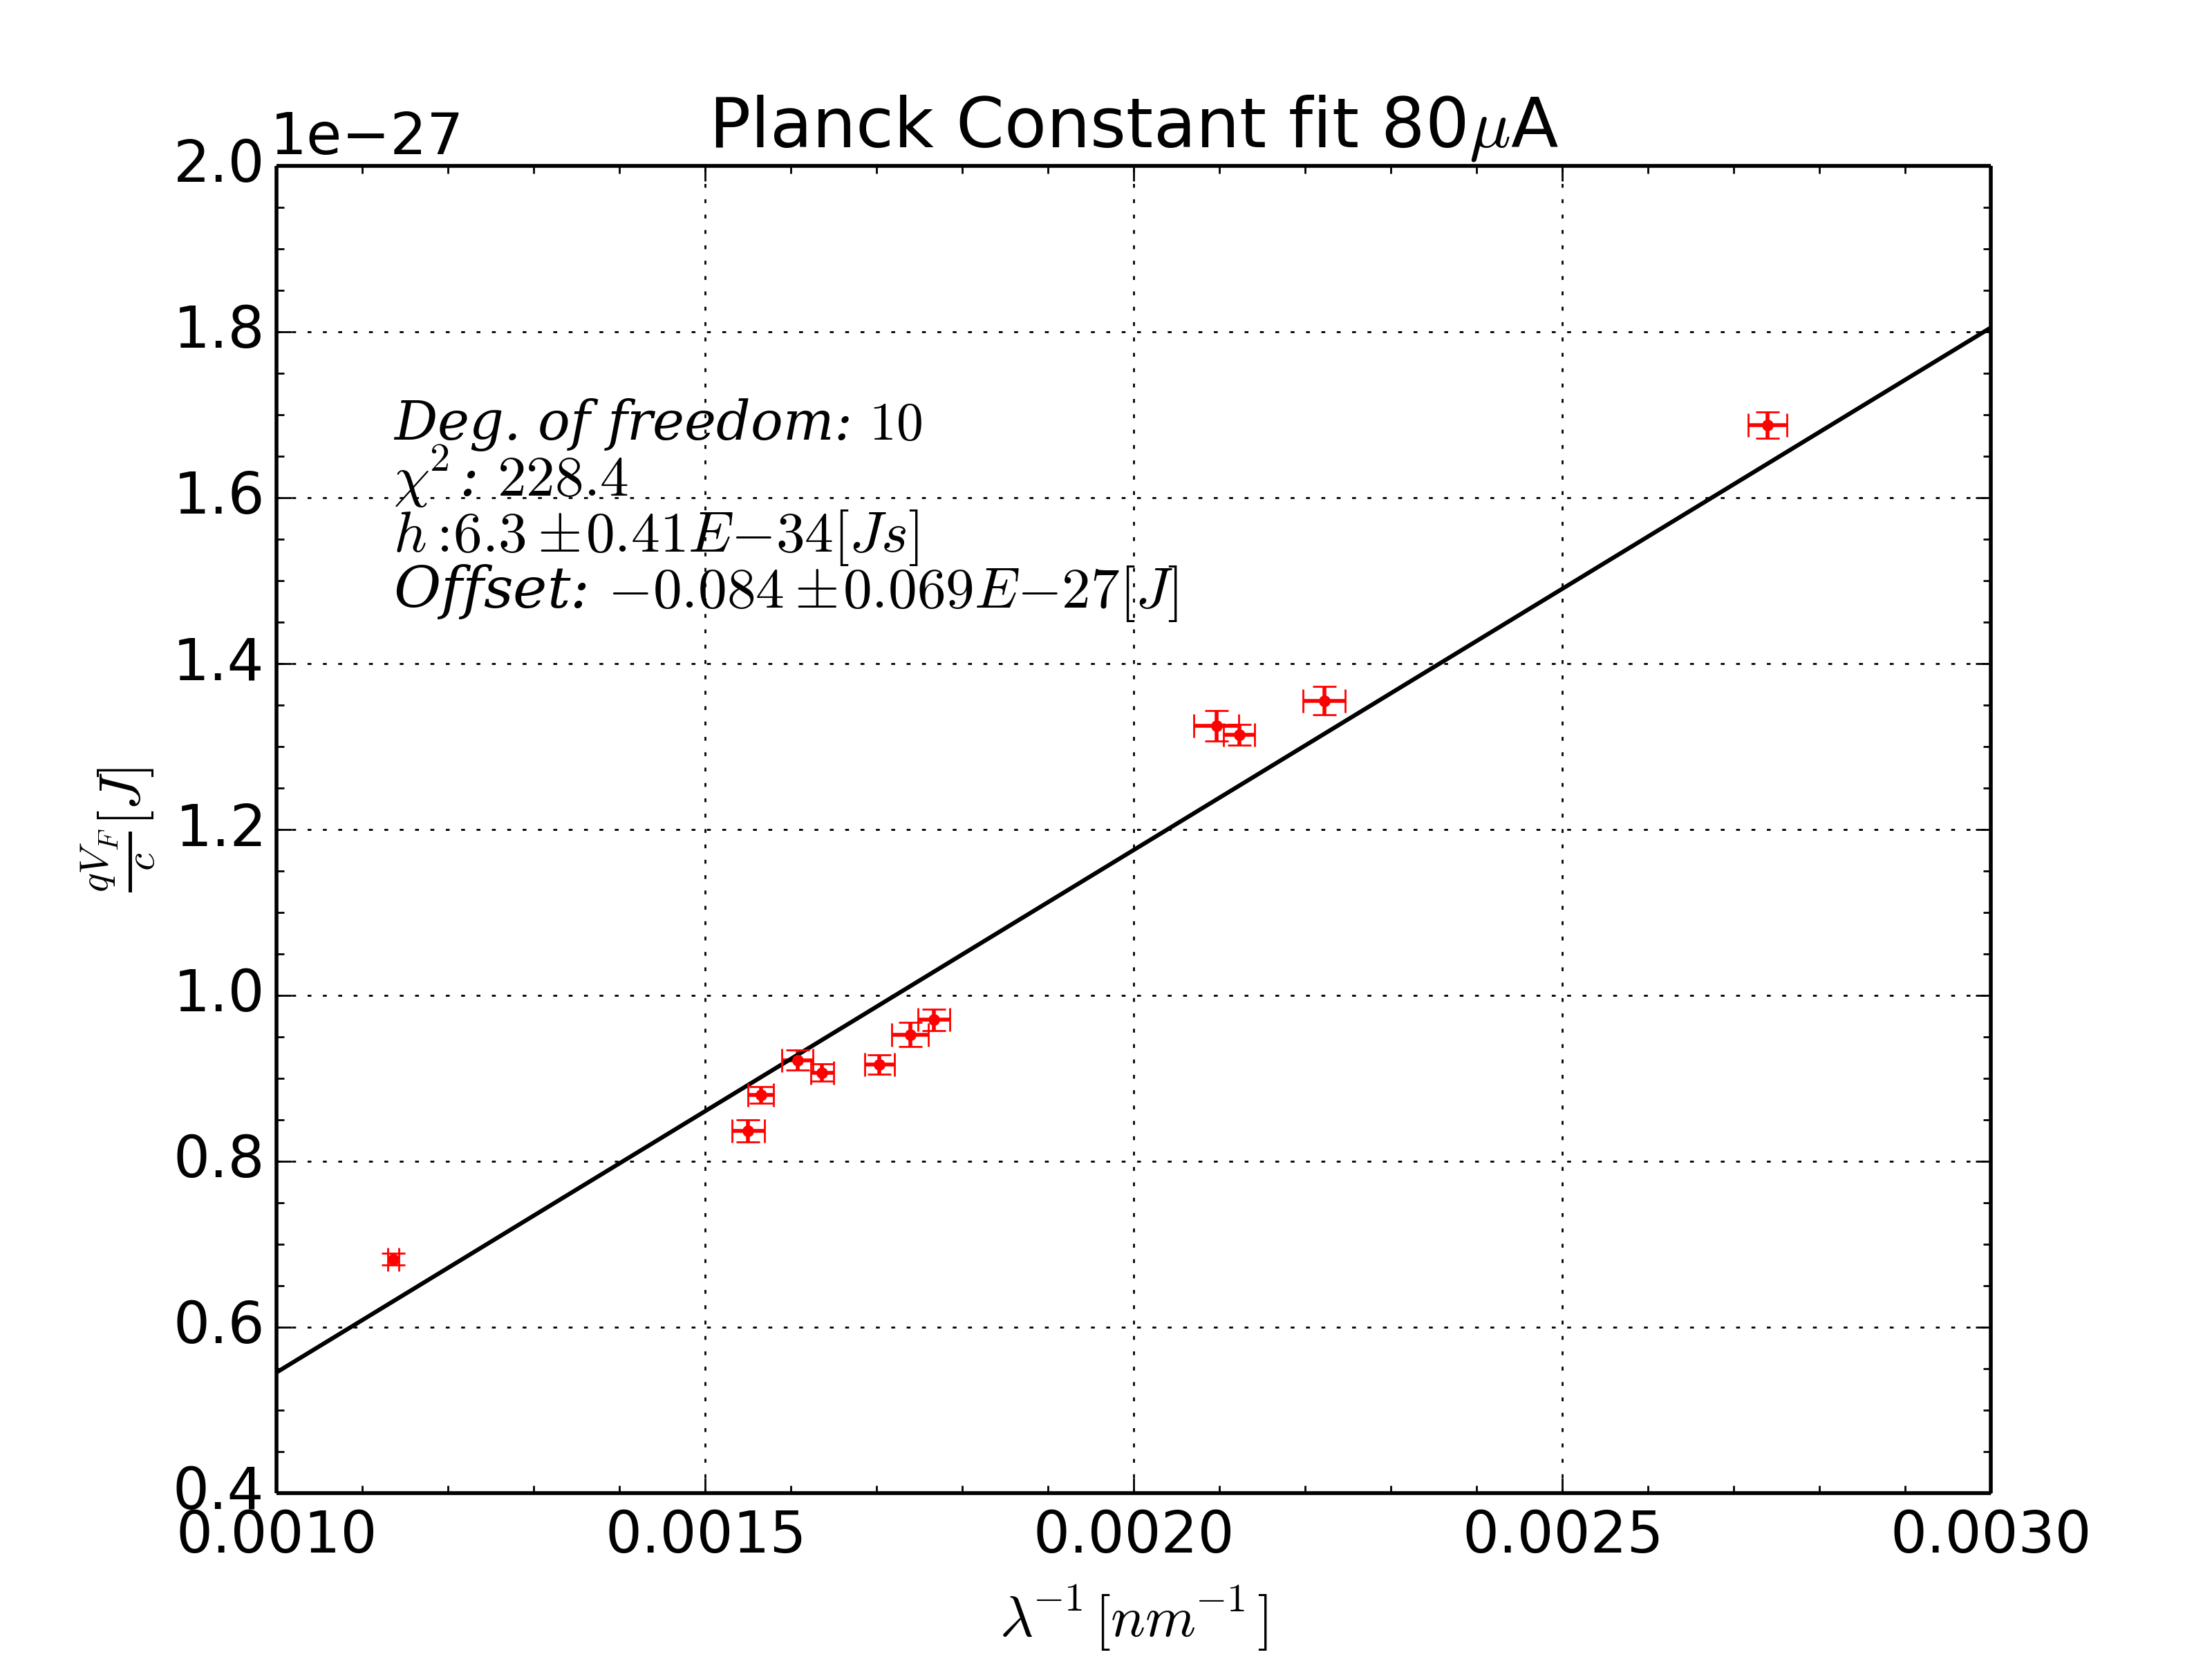
\includegraphics[width=0.9\linewidth]{./costante_planck_80ua}
\caption{Fit delle energie di gap in funzione del reciproco della lunghezza d'onda - 80 $\mu$A}
\label{fig:costante_planck_80ua}
\end{figure}

Il valore ricavato dal fit della costante di Planck è $6.30(41) \, E-34 \si{Js}$.

La conclusione che possiamo trarre è che, per quanto i valori di \textit{h} aumentino leggermente all'aumentare della corrente scelta per il "taglio", tale andamento risulta essere molto poco evidente rispetto a quanto ottenuto da altri gruppi, e anzi trascurabile.\\
Probabilmente ciò in una certa misura è dovuto al range di lavoro di corrente scelto e soprattutto dalla composizione del nostro set di LED.\\

Per convincercene, riportiamo in Figura (\ref{fig:costante_planck_comparison}) un grafico in cui sono riportate le rette restituite da tutti e quattro i fit, insieme con i punti sperimentali interpolati.

\begin{figure}
\centering
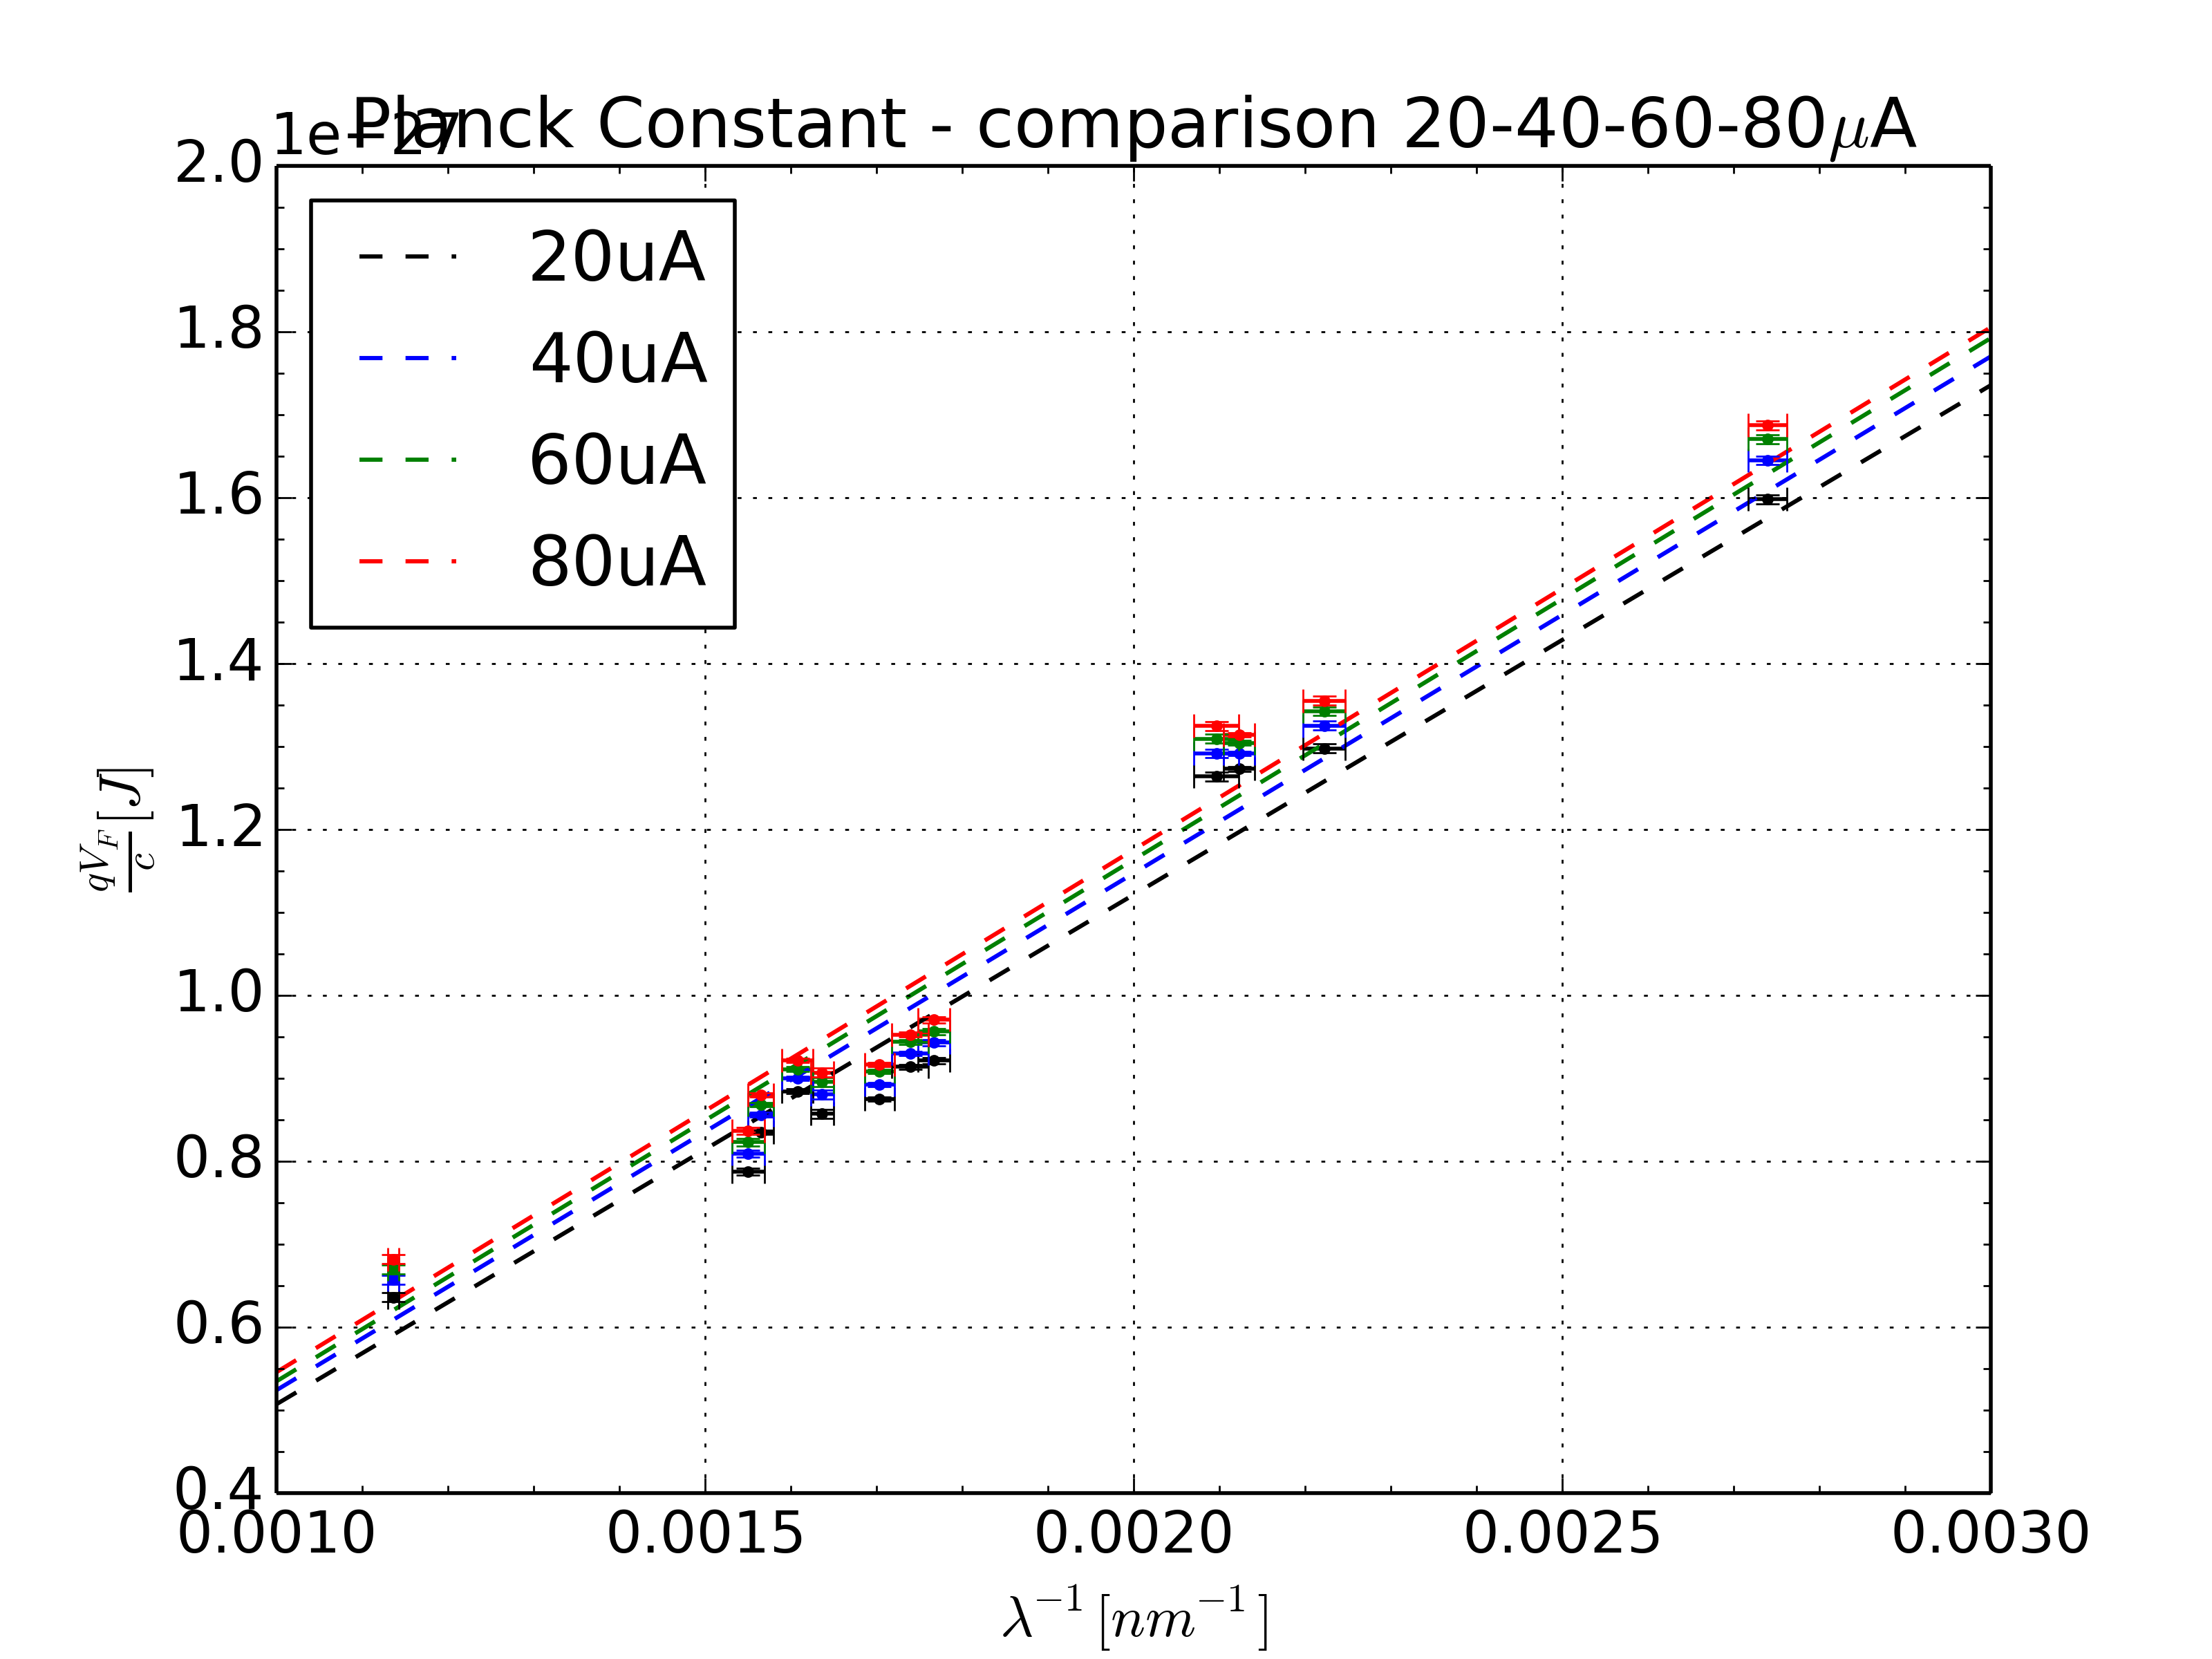
\includegraphics[width=0.9\linewidth]{./costante_planck_comparison}
\caption{Comparazione delle rette di fit per i diversi valori delle correnti. Si notino i punti interpolati nelle quattro condizioni.}
\label{fig:costante_planck_comparison}
\end{figure}

E' interessante notare come i punti interpolati siano quasi perfettamente impilati l'uno sull'altro, anche se ciò dipende molto dalla scala di rappresentazione: se andiamo a guardare gli scarti effettivi dalle tabelle di dati, si nota una certa variazione relativa delle tensioni di LED differenti all'aumentare delle correnti.

Per concludere la nostra analisi, è interessante a questo punto fittare solo i LED che abbiamo visto appartenere alla stessa "famiglia" e comportarsi "bene", per verificare che valore di \textit{h} ootteniamo. Il fit è riportato in Figura (\ref{fig:costante_planck_80ua_exclud1}).

\begin{figure}
\centering
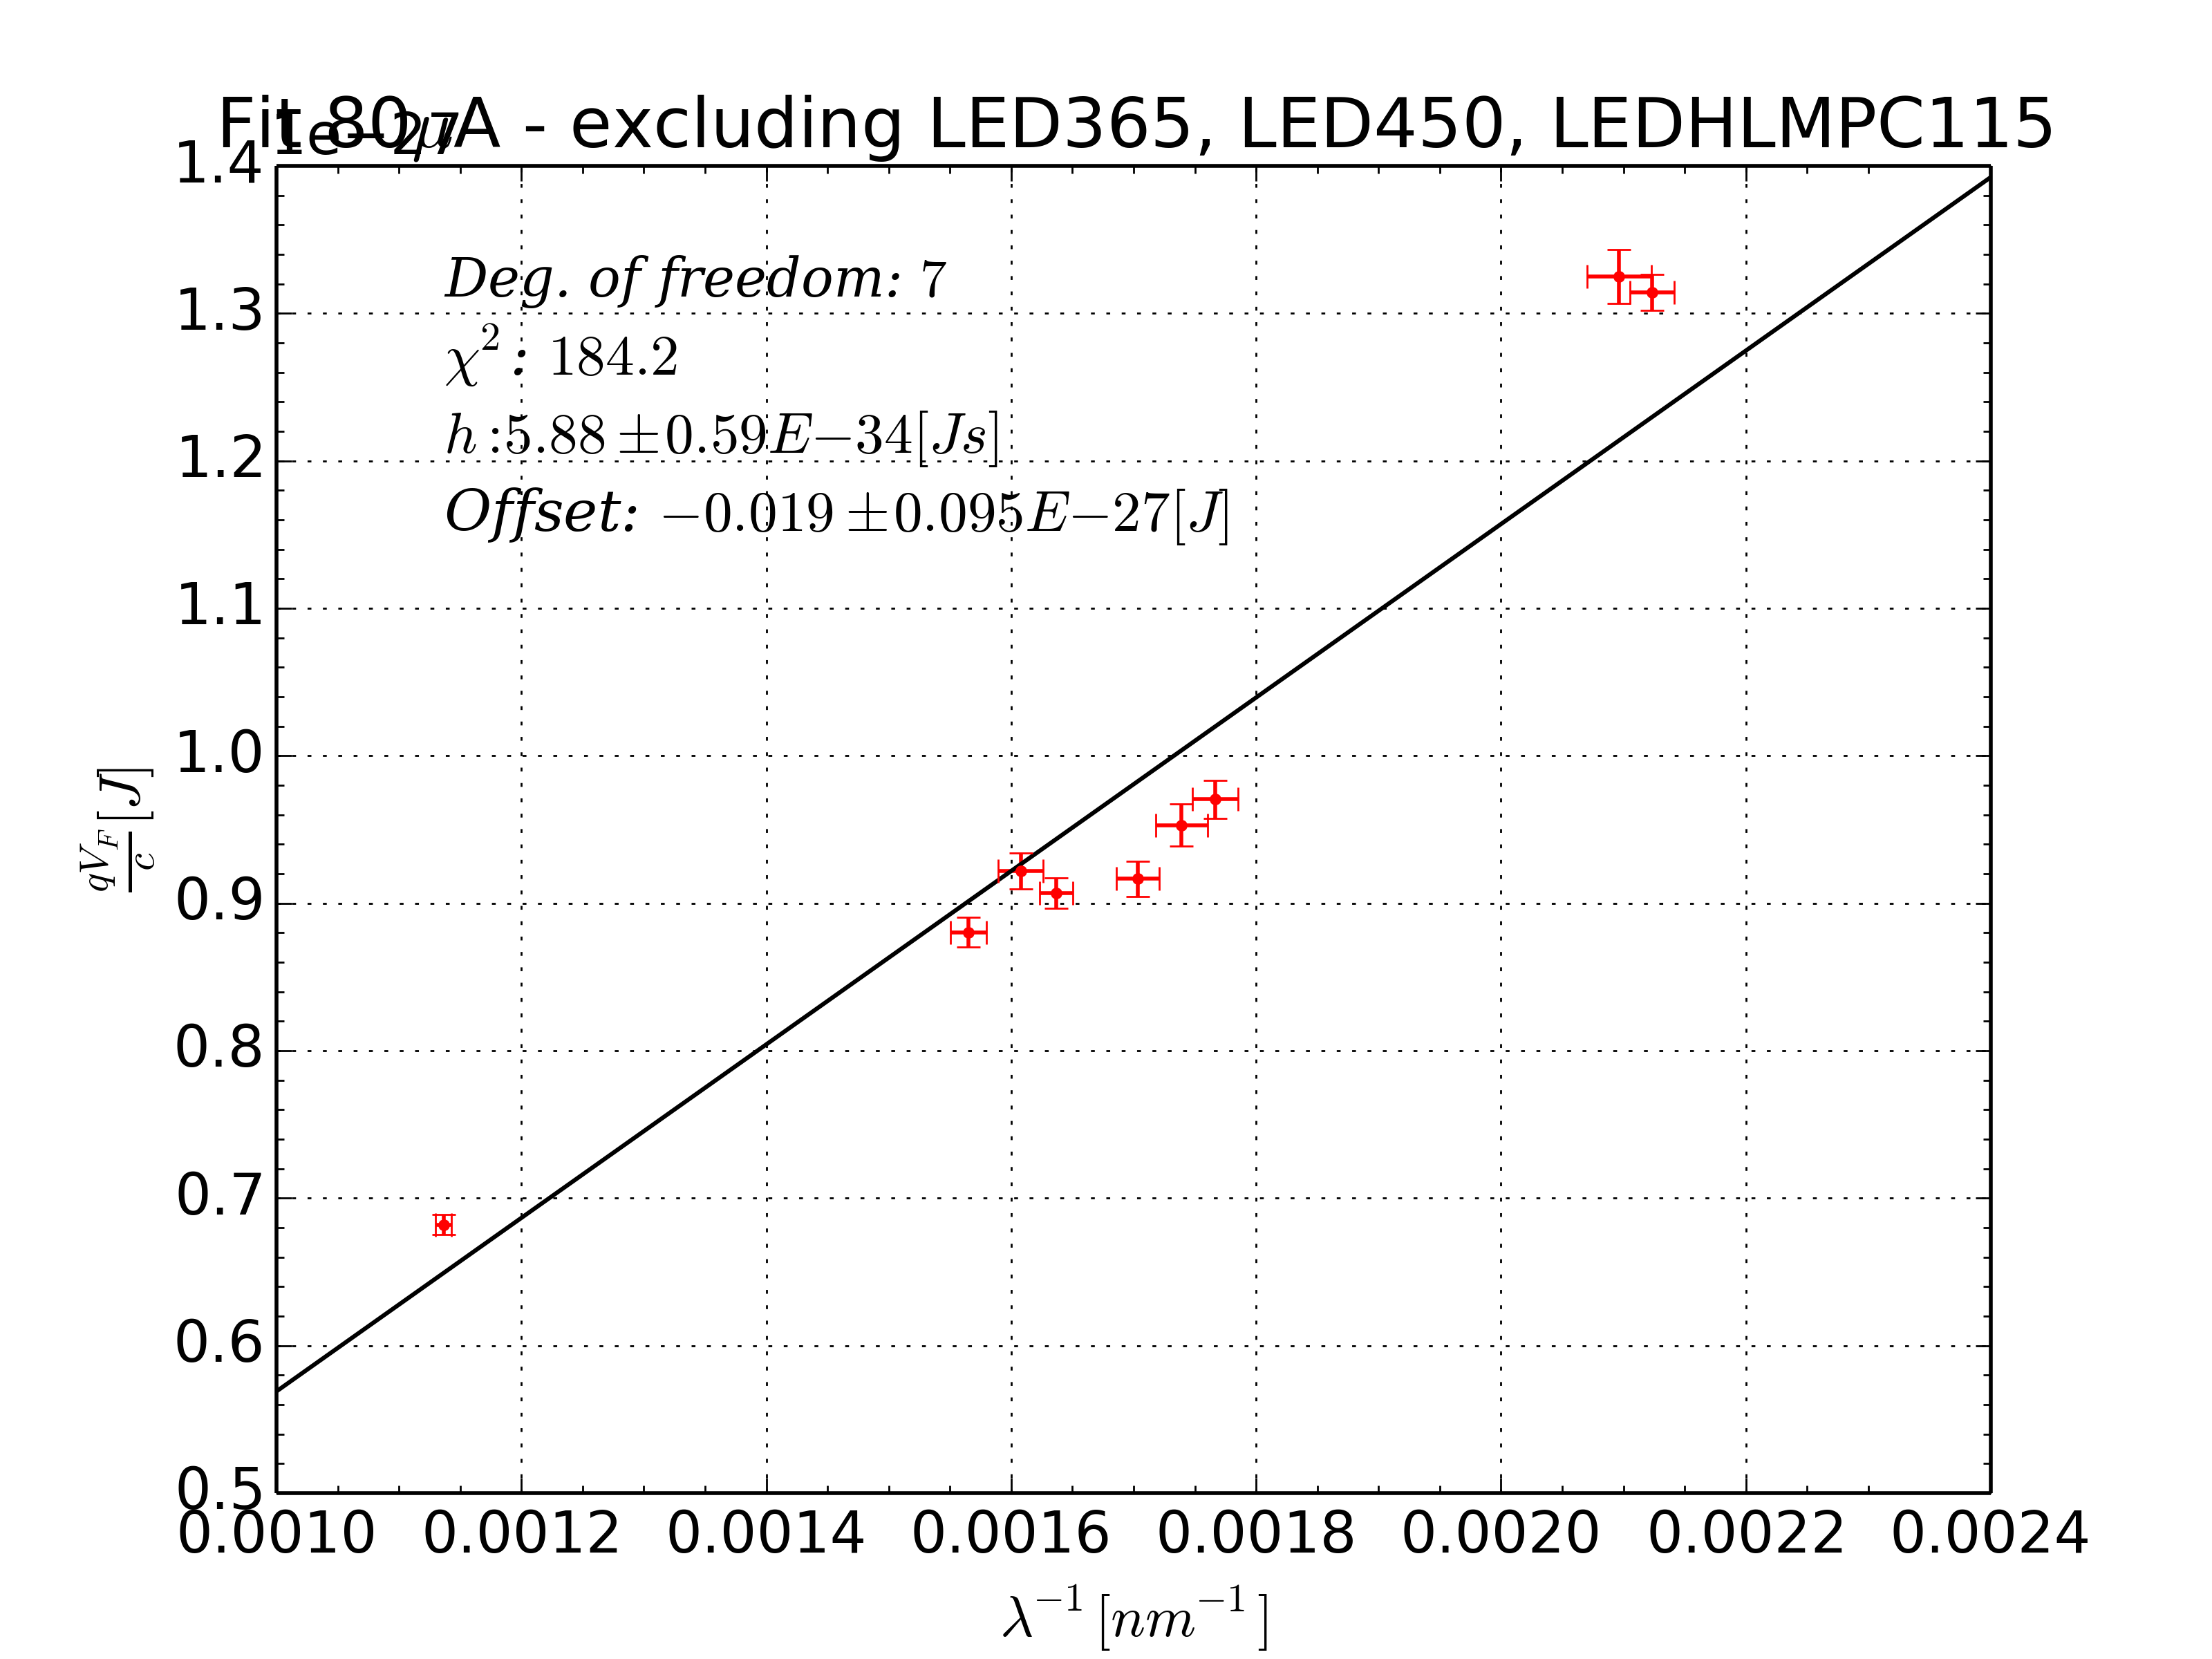
\includegraphics[width=0.9\linewidth]{./costante_planck_80ua_exclud1}
\caption{Fit della costante di Planck escludendo il LED365, LED450, HLMPC115.}
\label{fig:costante_planck_80ua_exclud1}
\end{figure}

Evidentemente, il risultato ($5.88(59) \, E-35 \si{Js}$)si discosta in maniera sostanziale dal valore conosciuto. Ed è proprio grazie ai LED "sospetti" che in realtà otteniamo un risultato più accurato! \\
Questo è indice del fatto che il modello che abbiamo proposto e impiegato per svolgere questa esperienza non è del tutto valido e esaustivo. \\
Inoltre, la presenza di gruppi di LED di dimensioni (a livello di numero di componenti) sensibilmente diverse, risulta in un peso differente che viene assegnato alle varie lunghezze d'onda esaminate; questo in particolar modo in base al comportamento già evidenziato dei diversi gruppi. Un modo per ridurre questa asimmetria consiste semplicemente nello scegliere dei LED equispaziati nel range di $\lambda$, in modo che queste siano pesate ugualmente.



\begin{thebibliography}{5}

	%Each item starts with a \bibitem{reference} command and the details thereafter.
	\bibitem{HOP96} % Transaction paper
	Datasheet, $\mu $A741 General-Purpose Operational Amplifiers. SLOS094E – NOVEMBER 1970  –REVISED JANUARY 2015.
	\url{http://www.ti.com/lit/ds/symlink/ua741.pdf}

	\bibitem{MJ06} % Conference paper
	Product data sheet: 1N4148 High-speed diodes. NXP Semiconductors 2004 Aug 10.
	\url{http://www.nxp.com/documents/data_sheet/1N4148_1N4448.pdf}

	\bibitem{MJH0} % Conference paper
	Product data sheet: AD711 op-amp.
	\url{http://www.analog.com/media/en/technical-documentation/data-sheets/AD711.pdf}
	
	\bibitem{JH06} % Conference paper
	Product data sheet: OP27 op-amp.
	\url{http://www.analog.com/media/en/technical-documentation/data-sheets/OP27.pdf}
	
	\bibitem{JH6} % Conference paper
	Product data sheet: tl081 op-amp.
	\url{http://www.ti.com/lit/ds/symlink/tl081.pdf}

	\bibitem{M06} % Conference paper
	Paul Horowitz, Winfield Hill - The Art of Electronics. Cambridge University Press (1989).
	
\end{thebibliography}

% Your document ends here!
\end{document}